% \section{METHODS}

% In order to simulate the transport of x-rays through a domain, the following is required:

% \begin{enumerate}
%     \item The geometry of the domain
%     \item The materials in the domain
%     \item The associated cross-sections, form factors, and scattering functions of the materials
%     \item The source of the x-rays (energy spectrum, position, and direction)
%     \item The number of photons to simulate
% \end{enumerate}

% and to retrieve information about the performed simulation, the following is required:

% \begin{enumerate}
%     \item Geometries to check for intersection
%     \item Quantities to tally
%     \item Derived quantities to calculate from tallied quantities
% \end{enumerate}

% \subsection{GEOMETRY}
% \par In MIDSX, the geometry of the domain is represented by a 3D array of voxels, with each voxel being assigned a material ID. The domain is assigned a particular size, indicated by its spatial extent along the x, y, and z dimensions. In addition, the domain is assigned a background material ID. Geometries inside the domain are specified by NIFTI files \cite{nifti2004}. These NIFTI files are assigned material IDs, spatial size, voxel size, and an origin, which is the location of the voxel in the domain that corresponds to the origin of the NIFTI file. After constructing the NIFTI files, the domain is defined by supplying the background material ID, domain size, and a list of NIFTI files into a custom .domain file, which is then read by the MIDSX executable. \\
% \par In the code, both a \code{VoxelGrid} and \code{ComputationalDomain} object are created, with the \code{ComputationalDomain} consisting of the specified dimensions, background material ID, and a vector of \code{VoxelGrid} objects which are created via the provided NIFTI files. Do determine the current material of a photon, it is first determined if the photon is inside the \code{ComputationalDomain}. If so, it then checks if the photon is inside any of the \code{VoxelGrid} objects. If so, it is then determined which Voxel the photon is located inside the Voxel, then the corresponding material ID is returned. If the photon is not inside the \code{ComputationalDomain}, then the photon is terminated. \\

% \subsection{MATERIALS \& DATA}
% \par In order to simulate the transport of x-rays through a domain, the materials in the domain must be specified. In MIDSX, materials are all defined in an SQLite database \cite{sqlite2020hipp}, which is read by the MIDSX executable. The database contains the following information for each element:

% \begin{enumerate}
%     \item Symbol
%     \item Atomic Number
%     \item Mass
%     \item Mass Density
%     \item Number Density
%     \item Mass Number
% \end{enumerate}

% All of the above data was obtained from the periodictable \cite{periodictable2022} and mendeleev \cite{mendeleev2021} python packages. In addition, the database contains the following data from the EPDL database \cite{cullen_survey_nodate} for each element:

% \begin{enumerate}
%     \item Total Microscopic Cross-Section
%     \item Photoelectric Microscopic Cross-Section
%     \item Coherent Scattering Microscopic Cross-Section
%     \item Incoherent Scattering Microscopic Cross-Section
%     \item Atomic Form Factor
%     \item Scattering Function
% \end{enumerate}

% \par In MIDSX, all the above data is initialized upon created creation of the \code{InteractionData} object with a vector of strings of materials names. These material names correspond to entries in the SQLite database, which contains a table of material compositions and mass densities which were obtained from NIST's mass attenuation coefficient database \cite{hubbell_x-ray_2004}. The \code{InteractionData} object contains a map of \code{Material} objects with their names, along with additional computed data, such as the maximum cross-section which is used for delta-tracking. The \code{Material} objects construct the above data for the specified material by performing an additivity approximation of the data for each element in the material as described by \cite{HUSSEIN2007153}. The data is separated into two further objects: \code{MaterialData} and \code{MaterialProperties}. \code{MaterialData} contains the microscopic cross-sections, form factors, and scattering functions, while \code{MaterialProperties} contains the mass density, number density, and mass.

% In addition to retrieving and storing the above data, the \code{MaterialData} object constructs interpolators for all its data. The interpolators for each type of data vary depending on its shape. For example, the photoelectric and total cross-sections are interpolated with a log-log linear interpolator, while the incoherent and coherent cross-sections are interpolated with a log-log cubic spline interpolator.

% \subsection{Source}
%     To generate the initial position, direction, and energy of a photon, a \code{PhotonSource} object is initialized with a \code{SourceGeometry}, \code{Directionality}, and an \code{EnergySpectrum} object. The three initializing object are virtual classes, allowing the user to specify the attributes of the source. The inheritance structure is shown in Fig (). 


% \subsection{Tallies}
% \par To measure simulation data, one must first decide when to trigger the measurement. In particular, MIDSX supports both surface and volume geometries that trigger when a photon passes through or enters the geometry, respectfully. For surfaces, users can choose discs and rectangles, while for volumes, there are only cuboids at the moment.
% \par At the start of the simulations, users can specify quantities that they want measured upon the trigger of a specific geometry. For surfaces, these include incident photon energy, entrance cosine, and number of photons, while for volumes, in addition to their own implementation of incident energy and number of photons, the quantities energy deposition and number of interactions are available for measurement. Furthermore, each quantity has the ability to specify between photons that underwent a single coherent scatter, a single incoherent scatter, multiple scatters, and no scatters. While this does noticeably increase the computation time, it was necessary to validate the interaction models used in MIDSX.
% \par At the end of simulation, one might want to calculate additional derived quantities from the tallied quantities from the simulation. With this mind, MIDSX contains a \code{DerivedQuantity} object that can calculate planar fluence and air kerma, which were implemented for half value layer experiments.
% \vspace{1cm}
% \par Using the described theory and methodology, the object \code{PhysicsEngine} transports a photon through the computational domain until termination. This process is described in Figure \ref{fig:PhysicsEngineFlowChart}.



% \begin{figure}[H]
%     \centering
% 	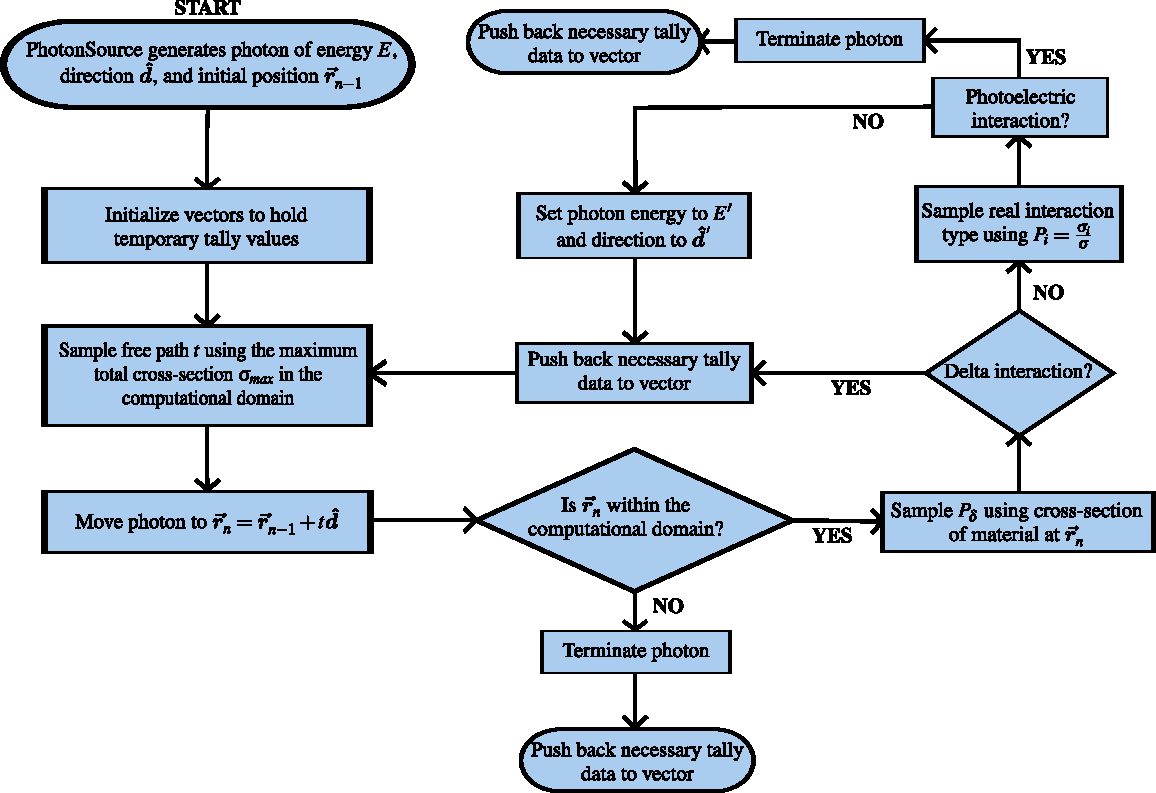
\includegraphics[width=1.0\textwidth]{../figures/physics_engine_flow_chart.pdf}
% 	\caption{Diagram of GE MiniView 6800 Mini C-Arm used in effective energy measurements.}
% 	\label{fig:PhysicsEngineFlowChart}
% \end{figure}

\section{IMPLEMENTATION}

\par To simulate x-ray transport in MIDSX, the domain's geometry is represented using a 3D voxel array with each voxel assigned a material ID. Geometries are defined by NIFTI files \cite{nifti2004} and incorporated into a custom .domain file. The code employs \code{VoxelGrid} objects which are contained within \code{ComputationalDomain} objects.
\par Materials are defined in an SQLite database \cite{sqlite2020hipp} containing elemental data from \cite{periodictable2022} and \cite{mendeleev2021}, and interaction data from the EPDL database \cite{cullen_survey_nodate}. The \code{InteractionData} object initializes this material data with various interpolation methods, including linear and spline interpolation.
\par The \code{PhotonSource} object, initialized with \code{SourceGeometry}, \code{Directionality}, and \code{EnergySpectrum}, determines the photon's initial attributes. MIDSX provides measurement triggers through surface and volume tallies. The geometries of these tallies correspond to regions of interest (ROI) and volumes of interest (VOI), respectively. Users can specify desired tally quantities via the \code{Quantity} and \code{QuantityContainer} objects, with post-simulation derived quantities like air kerma computed using the \code{DerivedQuantity} object.
\par For more details on the methodology used in MIDSX, see \cite{MIDSX2023}.

% \begin{figure}[H]
%     \centering
% 	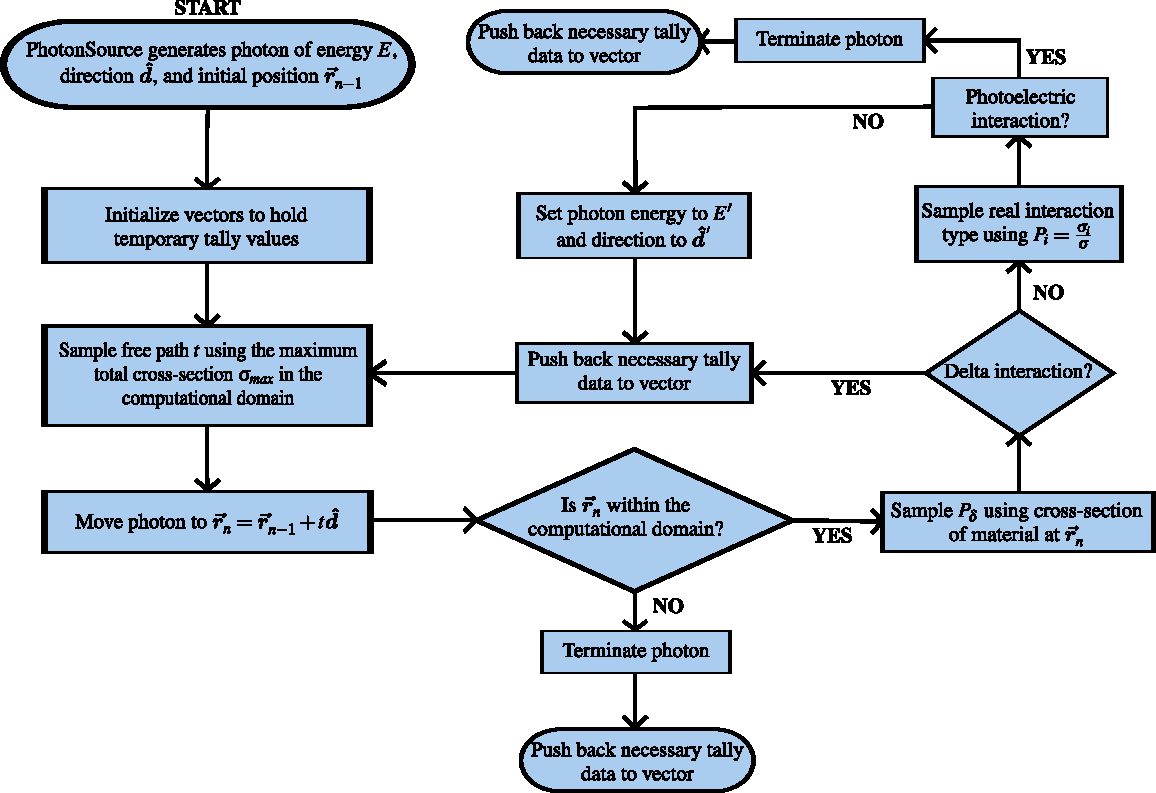
\includegraphics[width=0.9\textwidth]{../figures/physics_engine_flow_chart.pdf}
% 	\caption{Photon transport process in MIDSX.}
% 	\label{fig:PhysicsEngineFlowChart}
% \end{figure}
